\section{Iterator}

O padrão \textit{Iterator} traz uma forma de acessar ou 
percorrer objetos agregados sem expor sua representação. 
Isso é feito através de uma classe separada, o iterador, 
que implementa as operações necessárias para percorrer 
o objeto. \cite{gamma:1995}

Para que a classe cliente não precise conhecer o tipo 
da estrutura sendo percorrida, os objetos agregados 
são acessados através de uma interface. Também, para 
que não seja do cliente a responsabilidade de saber 
qual iterador instanciar, os objetos agregados devem 
definir uma operação que retorna o iterador adequado. 
Essa abordagem pode ser vista na Figura \ref{iterator_struct}, 
onde o cliente conhece apenas as interfaces 
\texttt{Aggregate} e \texttt{Iterator}.

\begin{figure}[htb]
	\caption{\label{iterator_struct}Estrutura do \textit{Iterator}.}
	\begin{center}
	    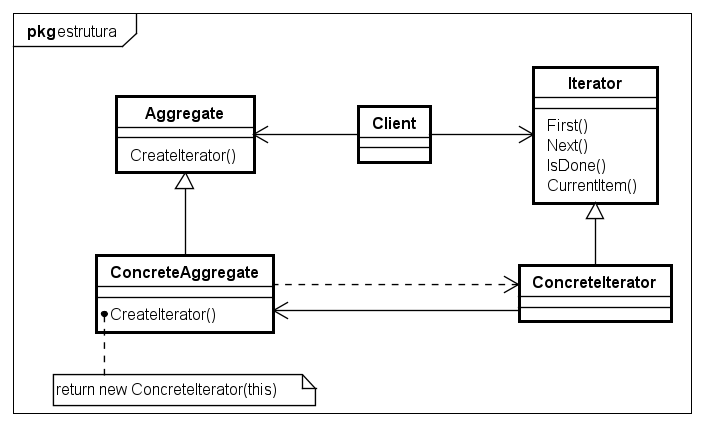
\includegraphics[scale=0.5]{5_padroes-contexto-funcional/5.3_comportamentais/5.3.04_iterator/iterator_struct.png}
	\end{center}
  \caption*{Fonte: O Autor (2021)}
\end{figure}

\subsection*{Exemplo Orientado a Objetos}

Como exemplo é desejado implementar um código 
que funcione para estruturas de lista comuns, mas 
que também funcione para \textit{skiplists}, uma 
estrutura de dados diferente que também se comporta 
como uma coleção. Para isso, é necessário que 
tanto as listas como as \textit{skiplists} implementem 
uma interface abstrata de lista, conhecida pela 
classe cliente. Da mesma forma, um iterador diferente 
é definido para cada um dos tipos, também de forma 
abstrata para o cliente. A Figura \ref{iterator_exemplo} 
demonstra o diagrama de classes para o exemplo, com a 
implementação no Código \ref{ooiterator}.

\begin{figure}[htb]
	\caption{\label{iterator_exemplo}Exemplo de \textit{Iterator}.}
	\begin{center}
	    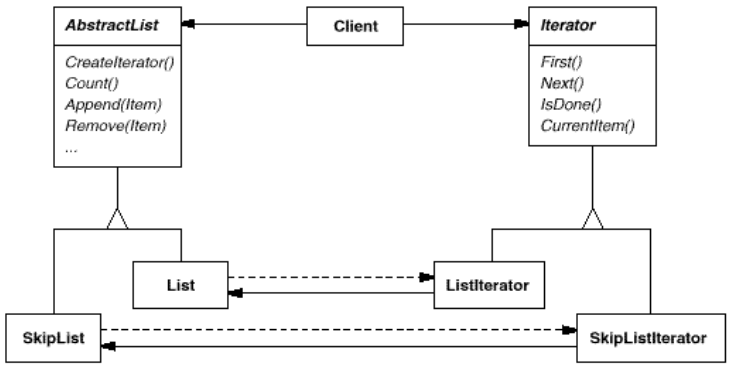
\includegraphics[scale=0.5]{5_padroes-contexto-funcional/5.3_comportamentais/5.3.04_iterator/iterator_exemplo.png}
	\end{center}
  \caption*{Fonte: O Autor (2021)}
\end{figure}

\begin{lstlisting}[caption={\textit{Iterator} Orientação a Objetos.},label=ooiterator]

trait AbstractList[A] {
  def CreateIterator() : Iterator[A]
  def Count() : Int
  def AppendItem(item : A)
  def RemoveItem(item : A)
}

class SimpleList[A] extends AbstractList[A] {

  private var elements : List[A] = List()

  def GetItem(pos : Int) : A = elements(pos)

  def CreateIterator(): Iterator[A] = new ListIterator[A](this)

  def Count(): Int = //Implementação para listas simples

  def AppendItem(item: A): Unit = {
    //Implementação para listas simples
  }
  def RemoveItem(item: A): Unit = {
    //Implementação para listas simples
  }
}

class SkipList[A] extends AbstractList[A] {

  def GetItem(pos : Int) : A = //Implementação para SkipLists

  override def CreateIterator(): Iterator[A] = new SkipListIterator[A]()

  override def Count(): Int = //Implementação para SkipLists

  override def AppendItem(item: A): Unit = {
    //Implementação para SkipLists
  }

  override def RemoveItem(item: A): Unit = {
    //Implementação para SkipLists
  }
}

trait Iterator[A] {
  def First() : A
  def Next() : A
  def IsDone() : Boolean
  def CurrentItem() : A
}

class ListIterator[A](elements : SimpleList[A]) extends Iterator[A] {
  private var pos : Int = 0
  private val list : SimpleList[A] = elements

  override def First(): A = list.GetItem(0)

  override def Next(): A = {
    if(pos+1<elements.Count()){
      pos = pos+1
    }
    elements.GetItem(pos)
  }

  override def IsDone(): Boolean = pos == elements.Count()

  override def CurrentItem(): A = elements.GetItem(pos)
}

class SkipListIterator[A](elements : SkipList[A]) extends Iterator[A] {
  private var pos : Int = 0
  private val list : SkipList[A] = elements

  override def First(): A = list.GetItem(0)

  override def Next(): A = {
    if(pos+1<elements.Count()){
      pos = pos+1
    }
    elements.GetItem(pos)
  }

  override def IsDone(): Boolean = pos == elements.Count()

  override def CurrentItem(): A = elements.GetItem(pos)
}
    
\end{lstlisting}
\legend{Fonte: O Autor (2021)}

\subsection*{Contexto Funcional}

O tipo de iterador apresentado no padrão pode 
ser considerado um \textit{Iterator} externo, onde a 
resposabilidade de acessar o elemento atual, 
passar para o próximo elemento ou verificar se 
a coleção terminou é da classe cliente. Por 
outro lado, um \textit{Iterator} interno funciona de forma 
que o cliente precisa apenas especificar qual 
operação deve ser executada, enquanto a 
coleção fica responsável por definir como ela 
deve ser percorrida. Essa abordagem de \textit{Iterator} 
pode ser alcançada através de funções como  
\textit{map} e \textit{reduce}\footnote{Também 
chamada de \textit{fold}}, que percorrem coleções 
de elementos enquanto executam uma função 
passada por parâmetro.\cite{iteratoressence}

O Código \ref{fpiterator} demonstra a definição 
das funções \texttt{Map} e \texttt{Reduce}. 
Na função \texttt{Map}, definida 
na linha 2, são recebidos como parâmetro uma 
função e uma lista de elementos de um tipo 
genérico \texttt{A}. A função recebida recebe um valor 
do tipo \texttt{A} e retorna um valor do tipo \texttt{B}. A função 
\texttt{Map} percorre todos os elementos da lista e 
aplica a função \textit{f} em todos os elementos, 
retornando uma nova lista do tipo \texttt{B}, cujos 
elementos são o resultado da aplicação de \textit{f} nos 
elementos da lista inicial.

Já na linha 9, é definida a função \texttt{Reduce}, que 
recebe como parâmetro uma função que recebe dois 
valores dos tipos \texttt{A} e \texttt{B} e retorna um valor do 
tipo \texttt{B}, um elemento acumulador do tipo \texttt{B} e uma 
lista de elementos do tipo \texttt{A}. O acumulador 
é um valor repassado pelas próximas iterações 
recursivas da função e sempre será o resultado 
da aplicação da função \textit{f} recebendo o elemento 
atual da lista e o acumulador recebido. 
Por fim, quando a lista acaba, é retornado o 
acumulador. 

\begin{lstlisting}[caption={Exemplos de \textit{Iterator}: \texttt{Map} e \texttt{Reduce}.},label=fpiterator]
    
def Map[A,B](f : A => B, elems : List[A]) : List[B] = {
  elems.head match {
    case Nil => Nil
    case e => f(e) :: Map(f, elems.tail)
  }
}

def Reduce[A,B](f : (A, B) => B, acc : B, elems : List[A]) : B = {
  elems.head match {
    case Nil => acc
    case e => Reduce(f, f(e, acc), elems.tail)
  }
}

\end{lstlisting}
\legend{Fonte: O Autor (2021)}

Da mesma forma que o \textit{Iterator} orientado a 
objetos visto no exemplo anterior, as funções 
\texttt{Map} e \texttt{Reduce} são genéricas em relação ao tipo 
de elemento armazenado pelas coleções. Da 
mesma forma, versões diferentes de \texttt{Map} e 
\texttt{Reduce} podem ser implementadas para tipos 
diferentes de coleção - da mesma forma que 
seriam implementadas classes diferentes de 
\textit{Iterator} para os tipos diferentes de listas 
no exemplo orientado a objetos. 
